\documentclass[11pt,class=report,crop=false]{standalone}
\usepackage[screen]{../python}

\begin{document}


%====================================================================
\chapitre{Tortue (Scratch avec Python)}
%====================================================================

\objectifs{Le module \ci{turtle}
 permet de tracer facilement des dessins en \Python{}. Il s'agit de commander une tortue à l'aide d'instructions simples comme \og{}avancer\fg{}, \og{}tourner\fg{}\ldots{} C'est le même principe qu'avec \emph{Scratch}, avec toutefois des différences : tu ne déplaces plus des blocs, mais tu écris les instructions ; et en plus les instructions sont en anglais !}


\insertvideo{OpJb6ur4JAk}{Tortue - partie 1}

\insertvideo{7Fb_FOp5NGs}{Tortue - partie 2}


%%%%%%%%%%%%%%%%%%%%%%%%%%%%%%%%%%%%%%%%%%%%%%%%%%%%%%%%%%%%%%%%
%%%%%%%%%%%%%%%%%%%%%%%%%%%%%%%%%%%%%%%%%%%%%%%%%%%%%%%%%%%%%%%%

\begin{cours}[La tortue \Python]
\index{module!turtle@\ci{turtle}}
\index{turtle@\ci{turtle}}
\index{tortue}
\index{graphique}

La tortue c'est l'ancêtre de \emph{Scratch} ! En quelques lignes tu peux faire de beaux dessins.

\begin{lstlisting}
from turtle import *

forward(100)  # On avance
left(90)      # 90 degrés à gauche
forward(50)
width(5)      # Epaisseur du trait
forward(100)
color('red')
right(90)
forward(200)

exitonclick()
\end{lstlisting}

\begin{center}
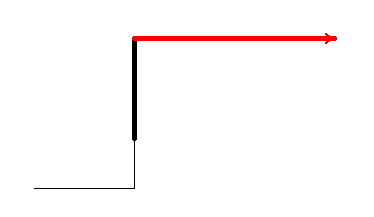
\includegraphics[scale=0.6]{ecran-tortue-0}
\end{center}

Voici une liste des principales commandes, accessibles après avoir écrit :\\
\centerline{\ci{from turtle import *}}

\begin{itemize}
  \item \ci{forward(longueur)}\index{forward@\ci{forward}} avance d'un certain nombre de pas
  \item \ci{backward(longueur)} recule
  \item \ci{right(angle)}\index{right@\ci{right}} tourne vers la droite (sans avancer) selon un angle donné en degrés
  \item \ci{left(angle)}\index{left@\ci{left}} tourne vers la gauche
  \item \ci{setheading(direction)} s'oriente dans une direction ($0$ = droite, $90$ = haut, $-90$ = bas, $180$ = gauche)
  \item \ci{goto(x,y)}\index{goto@\ci{goto}} se déplace jusqu'au point $(x,y)$
  \item \ci{setx(newx)} change la valeur de l'abscisse
  \item \ci{sety(newy)} change la valeur de l'ordonnée
  
  
  \item \ci{down()}\index{down@\ci{down}} abaisse le stylo
  \item \ci{up()}\index{up@\ci{up}} relève le stylo
  \item \ci{width(epaisseur)} change l'épaisseur du trait
  \item \ci{color(couleur)} change la couleur : \ci{"red"}, \ci{"green"}, \ci{"blue"}, \ci{"orange"}, \ci{"purple"},\ldots
  
  \item \ci{position()}  renvoie la position $(x,y)$ de la tortue
  \item \ci{heading()} renvoie la direction \ci{angle} vers laquelle pointe la tortue
  \item \ci{towards(x,y)} renvoie l'angle entre l'horizontale et le segment commençant à la tortue et finissant au point $(x,y)$
  \item \ci{exitonclick()} termine le programme dès que l'on clique
\end{itemize}

Les coordonnées de l'écran par défaut vont de $-475$ à $+475$ pour les $x$ et
de $-400$ à $+400$ pour les $y$ ; $(0,0)$ est au centre de l'écran.

\myfigure{0.9}{
  \tikzinput{coord}
}

\end{cours}


%%%%%%%%%%%%%%%%%%%%%%%%%%%%%%%%%%%%%%%%%%%%%%%%%%%%%%%%%%%%%%%%
% Activité 1
%%%%%%%%%%%%%%%%%%%%%%%%%%%%%%%%%%%%%%%%%%%%%%%%%%%%%%%%%%%%%%%%

\begin{activite}[Premiers pas]

\objectifs{Objectifs : tracer tes premiers dessins.}

Trace les premières lettres de \Python{}, par exemple comme ci-dessous.

\begin{center}
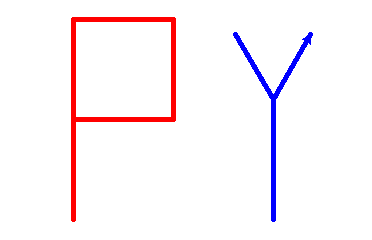
\includegraphics[scale=0.4]{ecran-tortue-1}
\end{center}

\end{activite}




%%%%%%%%%%%%%%%%%%%%%%%%%%%%%%%%%%%%%%%%%%%%%%%%%%%%%%%%%%%%%%%%
% Activité 2
%%%%%%%%%%%%%%%%%%%%%%%%%%%%%%%%%%%%%%%%%%%%%%%%%%%%%%%%%%%%%%%%

\begin{activite}[Figures]

\objectifs{Objectifs : tracer des figures géométriques.}

\begin{center}
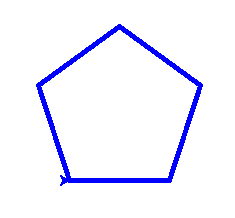
\includegraphics[scale=0.25]{ecran-tortue-2a}
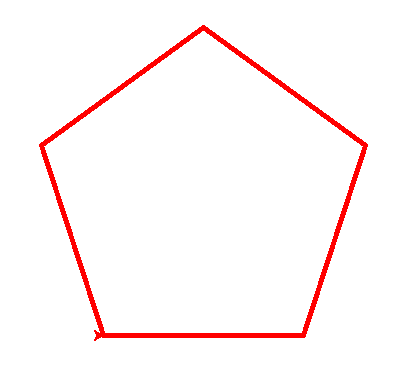
\includegraphics[scale=0.25]{ecran-tortue-2b}
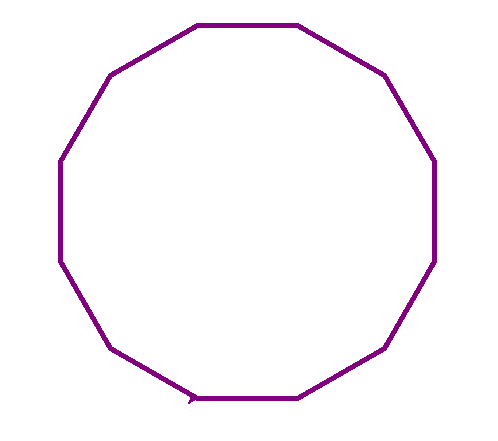
\includegraphics[scale=0.25]{ecran-tortue-2c}
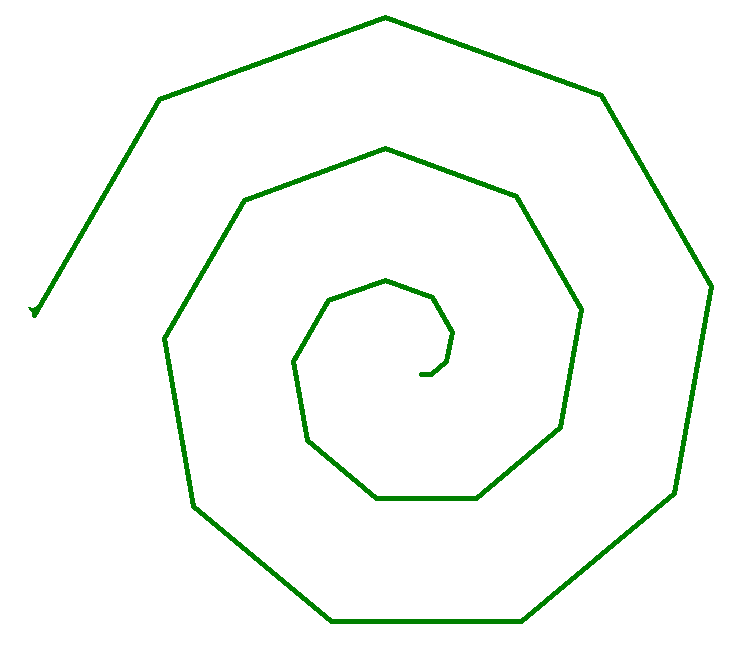
\includegraphics[scale=0.2]{ecran-tortue-2d}
\end{center}

\begin{enumerate}
  \item \textbf{Pentagone.} Trace un premier pentagone (en bleu). Tu dois répéter $5$ fois : avancer de $100$ pas, tourner de $72$ degrés.
  
  \emph{Indication.} Pour construire une boucle utilise \\
  \centerline{\ci{for i in range(5):}}
   (même si tu n'utilises pas ensuite la variable \ci{i}).
  
  \item \textbf{Pentagone (bis).} Définis une variable \ci{longueur} qui vaut $200$ et une variable \ci{angle} qui vaut $72$ degrés. Trace un second pentagone (en rouge) en avançant cette fois de \ci{longueur} et en tournant de \ci{angle}.
  
  \item \textbf{Dodécagone.} Trace un polygone à $12$ côtés (en violet). 
  
  \emph{Indication.} Pour tracer un polygone à $n$ côtés, il faut tourner d'un angle de $360/n$ degrés.
  
  \item \textbf{Spirale.} Trace une spirale (en vert).
  
  \emph{Indication.} Construis une boucle, dans laquelle tu tournes toujours du même angle, mais par contre tu avances d'une longueur qui augmente à chaque étape.
  
\end{enumerate}
  
\end{activite}



%%%%%%%%%%%%%%%%%%%%%%%%%%%%%%%%%%%%%%%%%%%%%%%%%%%%%%%%%%%%%%%%
% Activité 3
%%%%%%%%%%%%%%%%%%%%%%%%%%%%%%%%%%%%%%%%%%%%%%%%%%%%%%%%%%%%%%%%

\begin{activite}[Graphe de fonctions]

\objectifs{Objectifs : tracer le graphe d'une fonction.}

\begin{center}
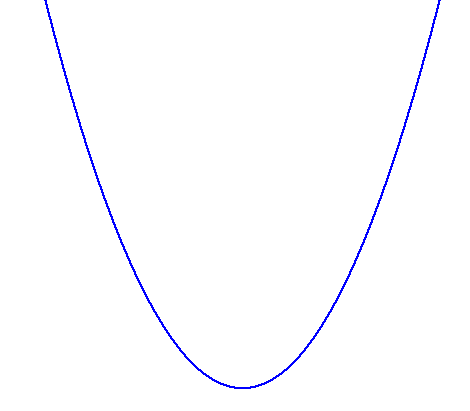
\includegraphics[scale=0.4]{ecran-tortue-3a}
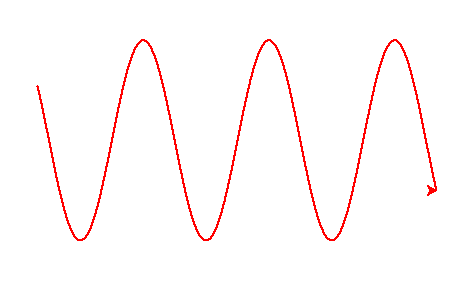
\includegraphics[scale=0.4]{ecran-tortue-3b}
\end{center}

Trace le graphe de la fonction carré et de la fonction sinus.

Afin d'obtenir une courbe dans la fenêtre de la tortue, répète pour $x$ variant de $-200$ à $+200$ :
\begin{itemize}
  \item poser $y = \frac{1}{100} x^2$,
  \item aller à $(x,y)$.
\end{itemize}

Pour la sinuso\"ide, tu peux utiliser la formule 
$$y = 100\sin\left(\frac{1}{20}x\right).$$
  
Par défaut \Python{} ne connaît pas la fonction sinus, pour utiliser \ci{sin()} il faut d'abord importer le module \ci{math} :\\
\centerline{\ci{from math import *}}

Pour que la tortue avance plus vite, tu peux utiliser la commande \ci{speed("fastest")}.
\end{activite}



%%%%%%%%%%%%%%%%%%%%%%%%%%%%%%%%%%%%%%%%%%%%%%%%%%%%%%%%%%%%%%%%
% Activité 4
%%%%%%%%%%%%%%%%%%%%%%%%%%%%%%%%%%%%%%%%%%%%%%%%%%%%%%%%%%%%%%%%

\begin{activite}[Triangle de Sierpinski]

\objectifs{Objectifs : tracer le début de la fractale de Sierpinski en imbriquant des boucles.}

\index{triangle de Sierpinski}

\begin{center}
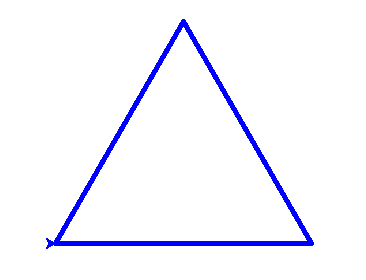
\includegraphics[scale=0.3]{ecran-tortue-4a}
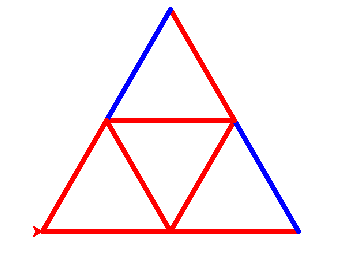
\includegraphics[scale=0.3]{ecran-tortue-4b}
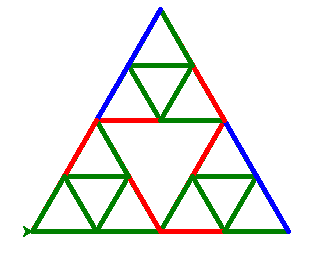
\includegraphics[scale=0.3]{ecran-tortue-4c}
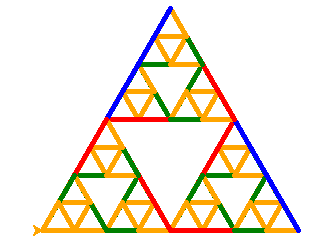
\includegraphics[scale=0.3]{ecran-tortue-4d}
\end{center}

Voici comment tracer le second dessin. Analyse l'imbrication des boucles et trace les dessins suivants.

\begin{center}
\begin{minipage}{0.5\textwidth}
\begin{lstlisting}
for i in range(3):
    color("blue")
    forward(256)
    left(120)

    for i in range(3):
        color("red")
        forward(128)
        left(120)
\end{lstlisting}        
\end{minipage}
\end{center}        
\end{activite}



%%%%%%%%%%%%%%%%%%%%%%%%%%%%%%%%%%%%%%%%%%%%%%%%%%%%%%%%%%%%%%%%
% Activité 5
%%%%%%%%%%%%%%%%%%%%%%%%%%%%%%%%%%%%%%%%%%%%%%%%%%%%%%%%%%%%%%%%

\begin{activite}[Le c\oe ur des tables de multiplication]

\objectifs{Objectifs : dessiner les tables de multiplication. Pour une introduction en vidéo voir 
\href{https://youtu.be/-X49VQgi86E}{\emph{la face cachée des tables de multiplication}} sur \emph{Youtube} par Micmaths.}

On fixe un entier $n$. On étudie la table de $2$, c'est-à-dire 
que l'on calcule $2 \times 0$, $2\times 1$, $2 \times 2$, jusqu'à $2 \times (n-1)$. En plus les calculs se feront modulo $n$. On calcule donc  
$$2 \times k \pmod{n} \qquad \text{ pour } k=0,1,\ldots,n-1$$

Comment dessiner cette table ?

On place sur un cercle $n$ points numérotés de $0$ à $n-1$.
Pour chaque $k\in \{0,\ldots,n-1\}$, on relie le point numéro $k$
et le point numéro $2\times k \pmod{n}$ par un segment. 

Voici le tracé, de la table de $2$, modulo $n=10$.

%\begin{center}
% 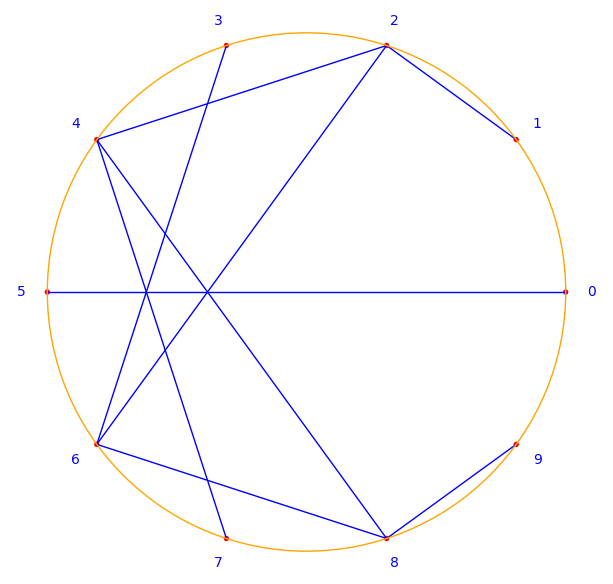
\includegraphics[scale=0.6]{fig-tortue-5a}  
%\end{center}

\myfigure{0.7}{
  \tikzinput{fig-tortue-5a}
}

Par exemple :
\begin{itemize}
  \item le point $3$ est relié au point $6$, car $2 \times 3 = 6$ ;
  \item le point $4$ est relié au point $8$, car $2 \times 4 = 8$ ;
  \item le point $7$ est relié au point $4$, car $2 \times 7 = 14 = 4 \pmod{10}$.
\end{itemize}

\bigskip

Trace la table de $2$ modulo $n$, pour différentes valeurs de $n$.



Voici ce que cela donne pour $n=100$.

\begin{center}
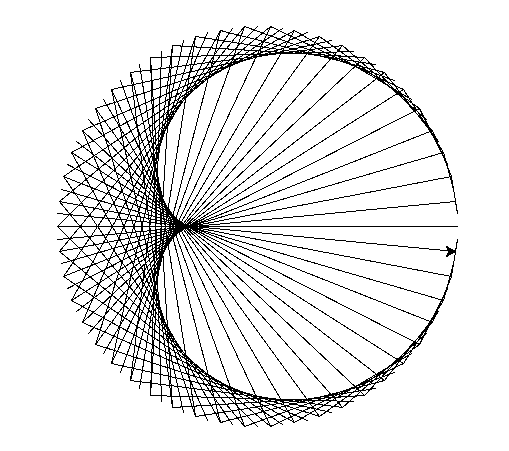
\includegraphics[scale=0.5]{ecran-tortue-5b}
\end{center}

\emph{Indications.}

Pour les calculs modulo $n$, utilise l'expression \ci{(2*k) \% n}.


Voici comment obtenir les coordonnées des sommets. Cela se fait avec les fonctions sinus et cosinus (disponibles à partir du module \ci{math}).
Les coordonnées $(x_i,y_i)$ du sommet numéro $i$, peuvent être calculées par la formule :
$$x_i = r \cos\left(\frac{2 i \pi}{n}\right) \qquad \text{ et } \qquad y_i = r\sin\left(\frac{2 i \pi}{n}\right)$$

Ces sommets seront situés sur le cercle de rayon $r$, centré en $(0,0)$. 
Tu devras choisir $r$ assez grand (par exemple $r=200$).


\myfigure{0.7}{
  \tikzinput{fig-tortue-5c}
}

\end{activite}

%%%%%%%%%%%%%%%%%%%%%%%%%%%%%%%%%%%%%%%%%%%%%%%%%%%%%%%%%%%%%%%%
%%%%%%%%%%%%%%%%%%%%%%%%%%%%%%%%%%%%%%%%%%%%%%%%%%%%%%%%%%%%%%%%

\begin{cours}[Plusieurs tortues]

On peut définir plusieurs tortues qui se déplacent de façon indépendante chacune de leur côté.
Voici comment définir deux tortues (une rouge et une bleue) et les déplacer.

\begin{lstlisting}
tortue1 = Turtle()   # Avec un 'T' majuscule !
tortue2 = Turtle()

tortue1.color('red')
tortue2.color('blue')

tortue1.forward(100)
tortue2.left(90)
tortue2.forward(100)
\end{lstlisting}

\end{cours}


%%%%%%%%%%%%%%%%%%%%%%%%%%%%%%%%%%%%%%%%%%%%%%%%%%%%%%%%%%%%%%%%
% Activité 6
%%%%%%%%%%%%%%%%%%%%%%%%%%%%%%%%%%%%%%%%%%%%%%%%%%%%%%%%%%%%%%%%

\begin{activite}[La poursuite des tortues]

\objectifs{Objectifs : tracer des courbes de poursuite.}


Programme quatre tortues qui courent les unes après les autres :

\begin{center}
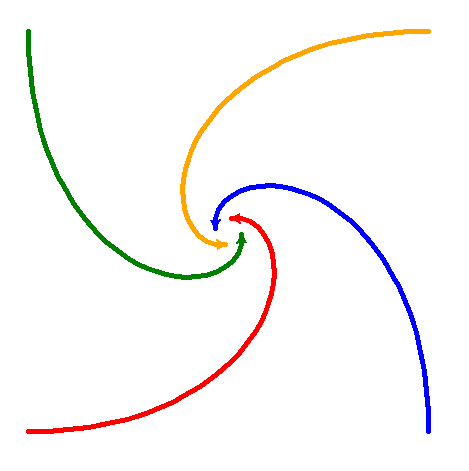
\includegraphics[scale=0.5]{ecran-tortue-6a}
\end{center}


\begin{itemize}
  \item la tortue 1 court après la tortue 2,
  \item la tortue 2 court après la tortue 3,
  \item la tortue 3 court après la tortue 4,
  \item la tortue 4 court après la tortue 1.
\end{itemize}

\bigskip

Voici les positions et orientations de départ :
\myfigure{0.9}{
\tikzinput{fig-tortue-6c}
}  


\emph{Indications.}
Utilise le bout de code suivant :
\begin{center}
\begin{minipage}{0.5\textwidth}
\begin{lstlisting}
position1 = tortue1.position()
position2 = tortue2.position()
angle1 = tortue1.towards(position2)
tortue1.setheading(angle1)
\end{lstlisting}
\end{minipage}
\end{center}
\begin{itemize}
  \item Tu places les tortues aux quatre coins d'un carré, par exemple en $(-200,-200)$,
  $(200,-200)$, $(200,200)$ et $(-200,200)$.
  \item Tu récupères la position de la première tortue  par 
  \ci{position1 = tortue1.position()}.
  Idem pour les autres tortues.
  \item Tu calcules l'angle entre la tortue 1 et la tortue 2 par la commande
  \ci{angle1 = tortue1.towards(position2)}.
  \item Tu orientes la tortue 1 selon cet angle :
  \ci{tortue1.setheading(angle1)}.
  \item Tu avances la tortue 1 de $10$ pas.
\end{itemize}

Améliore ton programme en traçant à chaque fois un segment entre la tortue poursuivante et la tortue poursuivie.

\begin{center}
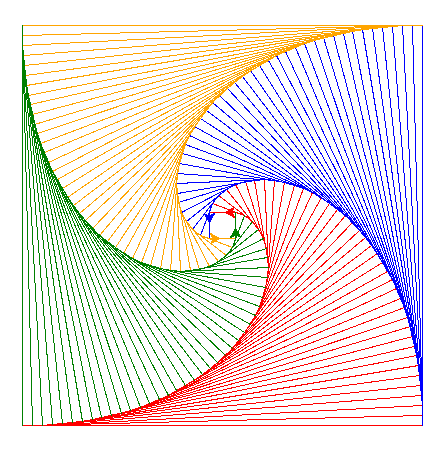
\includegraphics[scale=0.5]{ecran-tortue-6b}
\end{center}  
\end{activite}

\end{document}
